%% ============================================================================
%%  Physical Review B
%%  Emergent altermagnetic correlations and d_{xy} pairing in the checkerboard Hubbard model
%%
%%  Generated by code/build_manuscripts.py. Every number traces to a file in the
%%  repository; pointers are given in comments beside each claim.
%%  TODO before submission: author list, affiliations, acknowledgments, and the
%%  full bibliographic entry marked INCOMPLETE.
%% ============================================================================
\documentclass[aps,prb,reprint,superscriptaddress,amsmath,amssymb,floatfix]{revtex4-2}

\usepackage{graphicx}
\usepackage{bm}
\graphicspath{{../figures/}}

\begin{document}

\title{Emergent altermagnetic correlations and $d_{xy}$ pairing in the
checkerboard Hubbard model}

% TODO: author list and affiliations to be completed by the authors.
\author{[Author One]}
\affiliation{[Affiliation]}
\author{[Author Two]}
\affiliation{[Affiliation]}

\date{\today}

\begin{abstract}
We study the half-filled Hubbard model on the checkerboard lattice by
constrained-path quantum Monte Carlo. The Hamiltonian is spin independent, so the
two magnetic sublattices are related by a fourfold rotation rather than by a
translation, and any spin splitting of the momentum distribution must be
generated by the interaction. We find compensated spin-split correlations above a
finite interaction strength whose momentum-space polarization is odd under $C_4$
and even under the diagonal mirror at all 126 interacting parameter sets studied,
which identifies the $d_{xy}$ channel. A control calculation at vanishing lattice
anisotropy, where the model reduces to the square lattice and the splitting is
forbidden by symmetry, fixes the statistical floor of the order parameter at
$6.3(2)\times10^{-4}$ per site, two orders of magnitude below the measured signal.
The interaction-induced pairing vertex vanishes identically in the noninteracting
limit and is largest in the $d_{xy}$ channel over the same range of anisotropy
where the magnetic signal is $d_{xy}$. Magnetism and pairing therefore select the
same representation, which distinguishes this state from the $d_{x^2-y^2}$
pairing reported for the checkerboard lattice in the regime where the two models
coincide. Finite-size analysis up to $16\times16$ sites places the extrapolated
staggered moment below the resolution of the calculation, so the correlations
remain short ranged on the lattices studied.
\end{abstract}

\maketitle

% ---------------------------------------------------------------------------
\section{Introduction}
% ---------------------------------------------------------------------------

Altermagnets combine a vanishing net moment with a spin-split band structure, a
combination long assumed to require either ferromagnetism or spin-orbit
coupling~\cite{Smejkal2022a,Smejkal2022b,SmejkalCrystal,Mazin2021}. The symmetry
classification and the order-parameter description have since been put on a
group-theoretic footing~\cite{McClarty2024,Bhowal2024,Roig2024}, and the state has
been identified in MnTe~\cite{Krempasky2024,Lee2024,Hariki2025},
CrSb~\cite{Reimers2024}, and RuO$_2$~\cite{Feng2022,Fedchenko2024}, though the last
of these remains contested~\cite{Bai2024}. Proposals for altermagnetic
superconductivity have followed~\cite{Brekke2023,Ouassou2023,Zhu2023,Chakraborty2024}.
The splitting follows from the crystal
symmetry. The two opposite-spin sublattices are connected by a rotation rather
than by a translation or an inversion, so the spin degeneracy that a conventional
antiferromagnet enforces is absent.

Most microscopic models of this state build the splitting into the Hamiltonian,
usually through a spin-dependent hopping. The splitting is then present already
at zero interaction, and the question of whether interactions alone can produce
it is left open~\cite{Leeb2024}. The Lieb lattice, whose flat band makes the
interacting problem sharp~\cite{Lieb1989,Mielke1991,Tasaki1992}, has been studied
twice for this purpose, and both papers state the gap directly,
noting that unbiased studies establishing an altermagnet as the ground state of
an interacting Hamiltonian are lacking~\cite{Kaushal2025,Duerrnagel2025}. Both
use methods with a controlled range of validity, unrestricted Hartree-Fock with
exact diagonalization on small clusters in the first case and a functional
renormalization group treatment of the weak-coupling limit in the second.

The checkerboard lattice offers a route to the same physics without putting it in
by hand. It is a square lattice with diagonal bonds on alternating plaquettes, so
the two sublattices are exchanged by a fourfold rotation about a plaquette center
but by no translation. The hopping is spin independent and the interaction is a
uniform on-site Hubbard $U$. Any spin splitting therefore appears only once
magnetic correlations develop, which is the emergent route rather than the
built-in one.

We report constrained-path quantum Monte Carlo calculations for this model at
half filling on lattices from $8\times8$ up to $16\times16$ sites. Three results
follow. The momentum-resolved spin polarization is nonzero above a finite $U$ and
has $d_{xy}$ symmetry at every interacting parameter set we examined. A null
calculation at vanishing anisotropy, where symmetry forbids the signal, places
the statistical floor two orders of magnitude below the measured values. The
interaction-induced pairing vertex is largest in the $d_{xy}$ channel over the
same anisotropy range, so the magnetic and pairing instabilities lie in the same
representation.

% ---------------------------------------------------------------------------
\section{Model and method}
\label{sec:model}
% ---------------------------------------------------------------------------

We consider the single-band Hubbard model~\cite{Hubbard1963,Arovas2022},
\begin{equation}
H = \sum_{ij\sigma} t_{ij}\, c^{\dagger}_{i\sigma} c^{\phantom{\dagger}}_{j\sigma}
    + U \sum_i n_{i\uparrow} n_{i\downarrow},
\label{eq:H}
\end{equation}
with nearest-neighbor hopping $t_{ij} = t_0$ and diagonal hopping $t_1 + t_2$
along $(1,1)$ and $t_1 - t_2$ along $(1,-1)$ on one sublattice, the two exchanged
on the other. Energies are in units of $|t_0|$, and we set $t_0 = -1$ and
$t_1 = 0.3$ throughout. The anisotropy is parametrized by $\delta$ through
$t_2 = -\delta$, so that $\delta = 0$ restores the plain square lattice with
uniform second-neighbor hopping and the two sublattices become equivalent. All
calculations reported here are at half filling unless stated otherwise.

\begin{figure}[t]
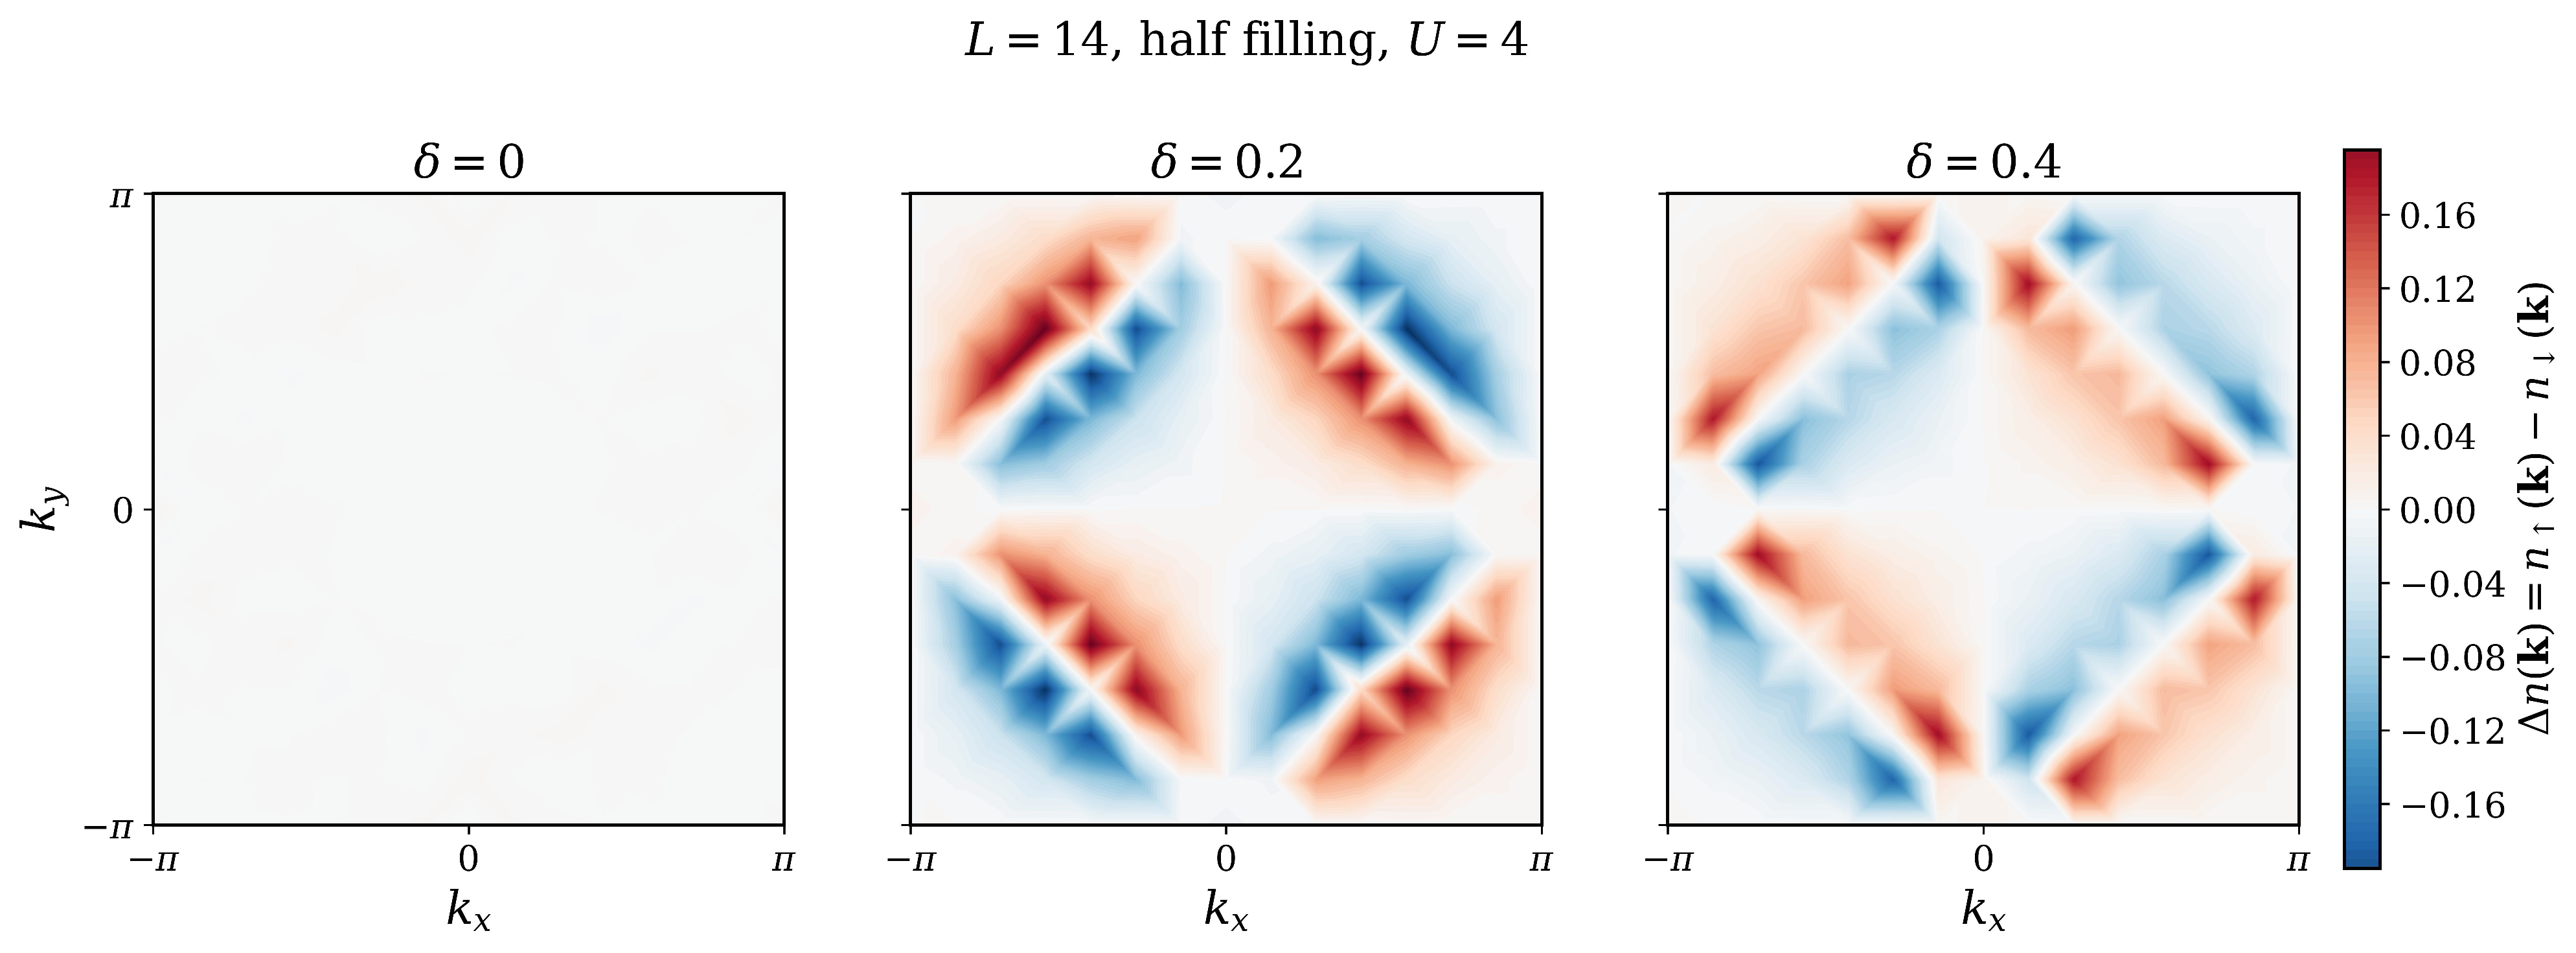
\includegraphics[width=\columnwidth]{1_dnk.pdf}
\caption{Checkerboard lattice and the mean-field spin polarization. The
nearest-neighbor hopping is $t$ and the diagonal hopping is $t_1 \pm \delta$ on
alternating plaquettes, with both spins seeing the same hopping. The momentum
distribution difference $\Delta n(\bm{k})$ vanishes at $\delta = 0$ and develops a
$d_{xy}$ pattern that grows with $\delta$ once a moment forms.}
\label{fig:model}
\end{figure}

The hopping in Eq.~(\ref{eq:H}) is spin independent by construction, so
$n_{\uparrow}(\bm{k}) = n_{\downarrow}(\bm{k})$ at $U = 0$ for every $\delta$.
Figure~\ref{fig:model} shows the geometry together with the mean-field
polarization it produces.

We use constrained-path quantum Monte Carlo
(CPQMC)~\cite{Zhang1997,ZhangKrakauer2003}, an auxiliary-field method~\cite{BSS1981,Hirsch1983,Sorella1989}
in which the constraint removes the exponential sign
problem~\cite{Loh1990,Troyer2005} at the cost of a bias. Benchmarks of the same
method against exact results for the square-lattice Hubbard model are
available~\cite{Hirsch1985,Varney2009,LeBlanc2015,Qin2016}. We use a Trotter step
$\Delta\tau = 0.01$, a projection length $\beta = 32$, and $N_w = 1000$ walkers.
The constrained-path approximation introduces a bias controlled by the trial wave
function, so we do not describe these results as exact. Appendix~\ref{app:trial}
sets out how the trial is chosen, which is not a neutral detail. Doubling the
projection length from $\beta = 32$ to $\beta = 48$ changes the order parameter by
between $0.1\%$ and $4.1\%$ with no systematic drift, which we take as
convergence in $\beta$.
% beta convergence: 32 -> 48 changes 0.1, 1.5, 2.4, 4.1 percent

\begin{figure}[t]
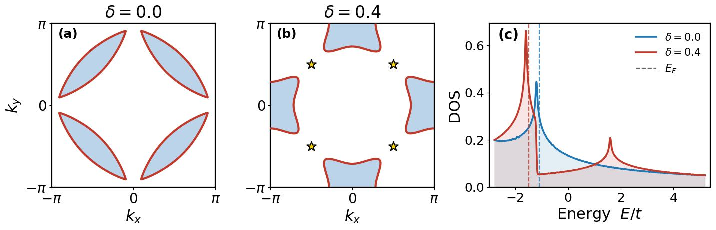
\includegraphics[width=\columnwidth]{2_vhs_dos.pdf}
\caption{Fermi surface and density of states of Eq.~(\ref{eq:H}) at $U = 0$. The
anisotropy $\delta$ moves the van Hove points to incommensurate momenta near the
Fermi level, which is the single-particle change that the interacting
calculations build on.}
\label{fig:vhs}
\end{figure}

The order parameter is the momentum-space spin polarization
\begin{equation}
\Delta_{\mathrm{tot}} = \sum_{\bm{k}} \left| n_{\uparrow}(\bm{k}) - n_{\downarrow}(\bm{k}) \right|,
\label{eq:dtot}
\end{equation}
following Ref.~\cite{OurPRB}. The absolute value inside the sum makes
$\Delta_{\mathrm{tot}}$ sensitive to a compensated splitting, for which the signed
sum $\sum_{\bm{k}} [n_{\uparrow}(\bm{k}) - n_{\downarrow}(\bm{k})]$ vanishes. We
quote $\Delta_{\mathrm{tot}}/N$ so that different lattice sizes can be compared,
and we note that Eq.~(\ref{eq:dtot}) as written in Ref.~\cite{OurPRB} is a bare
sum.

Because $H$ commutes with the total spin, the polarization must be induced by a
symmetry-breaking field. We add a staggered field $h$ that couples with opposite
sign to the two sublattices, which makes the trial state symmetry broken, and we
report the behavior as a function of $h$. The constrained path is defined by the
trial state, so this field biases the walkers toward the broken state, and the
control in Sec.~\ref{sec:null} is what establishes that the measured signal is
not an artifact of that bias.

To classify the symmetry of
$\Delta n(\bm{k}) = n_{\uparrow}(\bm{k}) - n_{\downarrow}(\bm{k})$ we use two
dimensionless ratios,
\begin{align}
A_{\mathrm{odd}} &= \frac{\sum_{\bm{k}} \left| \Delta n(\bm{k}) + \Delta n(R_{90}\bm{k}) \right|}
                         {\sum_{\bm{k}} \left| \Delta n(\bm{k}) \right|},
\label{eq:aodd}\\
M_{\mathrm{odd}} &= \frac{\sum_{\bm{k}} \left| \Delta n(\bm{k}) + \Delta n(M\bm{k}) \right|}
                         {\sum_{\bm{k}} \left| \Delta n(\bm{k}) \right|},
\label{eq:modd}
\end{align}
where $R_{90}$ is the fourfold rotation and $M$ the diagonal mirror
$(k_x,k_y) \to (k_y,k_x)$. A state odd under $C_4$ gives $A_{\mathrm{odd}} = 0$
and an even state gives $A_{\mathrm{odd}} = 2$. A $d_{x^2-y^2}$ state gives
$M_{\mathrm{odd}} = 0$ and a $d_{xy}$ state gives $M_{\mathrm{odd}} = 2$. These
ratios use only the symmetry of the data, so unlike a projection onto a single
lattice harmonic they are not sensitive to how the weight is distributed among
higher harmonics of the same symmetry.

% ---------------------------------------------------------------------------
\section{Emergent altermagnetic correlations}
\label{sec:order}
% ---------------------------------------------------------------------------

$\Delta_{\mathrm{tot}}$ vanishes identically at $U = 0$ and becomes finite for
$U > 0$ at every anisotropy studied, reaching $\Delta_{\mathrm{tot}}/N$ between
$2.2\times10^{-3}$ and $9.2\times10^{-2}$ over the interacting parameter sets.
% range from data/fortran_L12_all49.csv, U>0
The splitting is compensated, so the state carries momentum-resolved spin
polarization with no net moment. Figure~\ref{fig:dtot} shows the emergence over
the $(U,\delta)$ plane, with the $U = 0$ column exactly zero.

\begin{figure}[t]
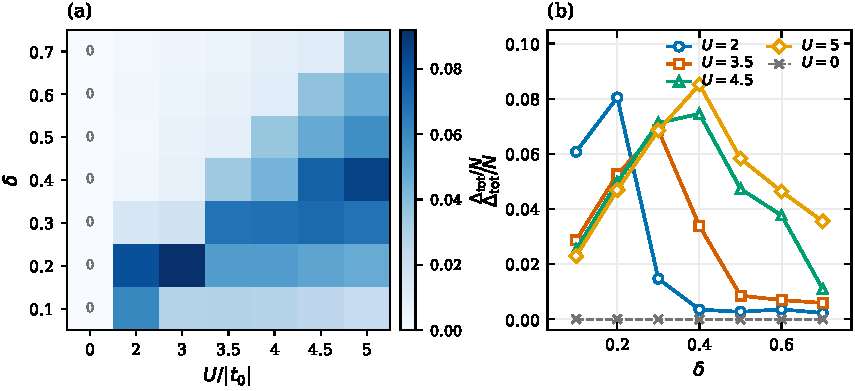
\includegraphics[width=\columnwidth]{fig03_dtot_emergence.pdf}
\caption{$\Delta_{\mathrm{tot}}/N$ over the $(U,\delta)$ plane at half filling.
The signal is identically zero along the $U = 0$ column and along $\delta = 0$,
where symmetry forbids it, and grows into the interior. Both zeros are required
by construction and neither was imposed.}
\label{fig:dtot}
\end{figure}

\begin{figure}[t]
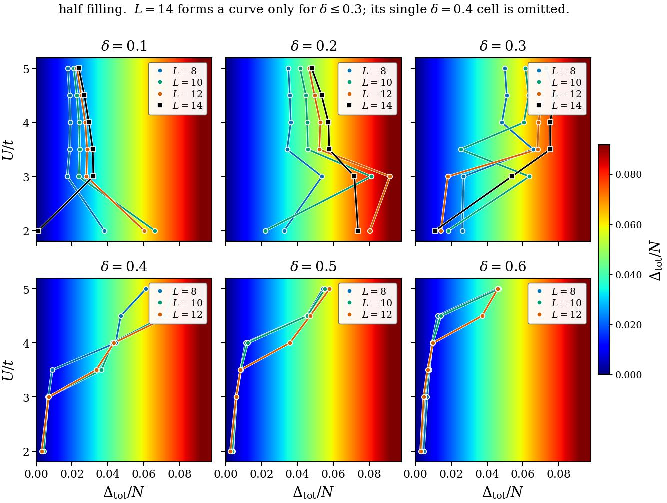
\includegraphics[width=\columnwidth]{fig_dtot_6delta.pdf}
\caption{$\Delta_{\mathrm{tot}}/N$ against $U$ at six anisotropies for
$L = 8$, $10$, $12$, and $14$. The background shades the same quantity on the
scale used in Fig.~\ref{fig:dtot}. The response is not monotonic in $\delta$, and
the strongest signal at fixed $U$ falls near $\delta = 0.4$.}
\label{fig:dtot6}
\end{figure}

The symmetry classification is unambiguous. Across all 126 interacting parameter
sets at $L = 8$, $10$, and $12$ we obtain $A_{\mathrm{odd}}$ between $0.004$ and
$0.263$ and $M_{\mathrm{odd}}$ between $1.24$ and $2.00$.
% data/classify_3L.csv, 126 cells
Restricted to $L = 12$ the ranges are $0.008$ to $0.166$ and $1.54$ to $2.00$.
% data/classify_L12.csv, 42 cells
The polarization is therefore odd under $C_4$ and even under the diagonal mirror
at every parameter set, which is the $d_{xy}$ channel. No parameter set is
classified as $d_{x^2-y^2}$. Figure~\ref{fig:symmetry} shows the two ratios
together with the rotation and mirror sums from which they are built.

\begin{figure}[t]
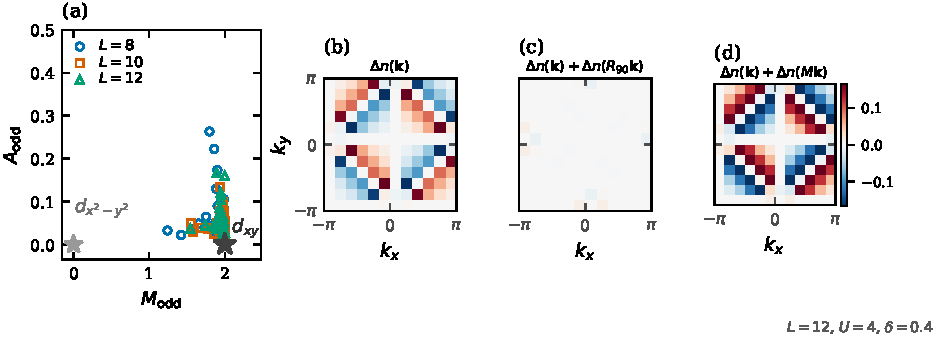
\includegraphics[width=\columnwidth]{fig04_symmetry.pdf}
\caption{Symmetry classification of $\Delta n(\bm{k})$. $A_{\mathrm{odd}}$ near
zero identifies a state odd under the fourfold rotation and $M_{\mathrm{odd}}$
near two identifies one even under the diagonal mirror, which together select
$d_{xy}$. The $C_4$ and mirror sums are shown directly alongside the ratios.}
\label{fig:symmetry}
\end{figure}

% ---------------------------------------------------------------------------
\section{What sets the size of the polarization}
\label{sec:mechanism}
% ---------------------------------------------------------------------------

The polarization is not monotonic in the anisotropy, which the order parameter
alone does not explain. Writing it as a product separates the two effects at
work. The altermagnetic order parameter can be decomposed as
\begin{equation}
m_{\mathrm{AM}} = \Delta m \, \delta ,
\label{eq:mam}
\end{equation}
where $\Delta m$ is the sublattice moment difference and $\delta$ the anisotropy
that converts it into a momentum-space splitting. Neither factor alone produces
the state. Without a moment there is nothing to split, and without the anisotropy
the two sublattices are related by a translation and the splitting is forbidden.

The two factors respond to the interaction in opposite ways.
Figure~\ref{fig:mam}(b) shows that $\Delta m$ grows from zero roughly linearly in
$U$ at every anisotropy, so the moment is built by the interaction alone.
Figure~\ref{fig:mam}(c) shows that $\Delta m$ falls monotonically with $\delta$ at
every interaction strength, by about a factor of three between $\delta = 0$ and
$\delta = 0.7$ at $U = 8$. The anisotropy that makes the splitting possible also
frustrates the magnetic order that supplies it.

The product in Eq.~(\ref{eq:mam}) therefore rises steeply at small $\delta$, where
the linear factor dominates, and flattens above $\delta \approx 0.3$, where the
suppression of $\Delta m$ compensates the growth of the prefactor
[Fig.~\ref{fig:mam}(d)]. This is the origin of the optimal anisotropy seen in the
maps of Sec.~\ref{sec:order}, and it is a competition rather than a resonance.

\begin{figure}[t]
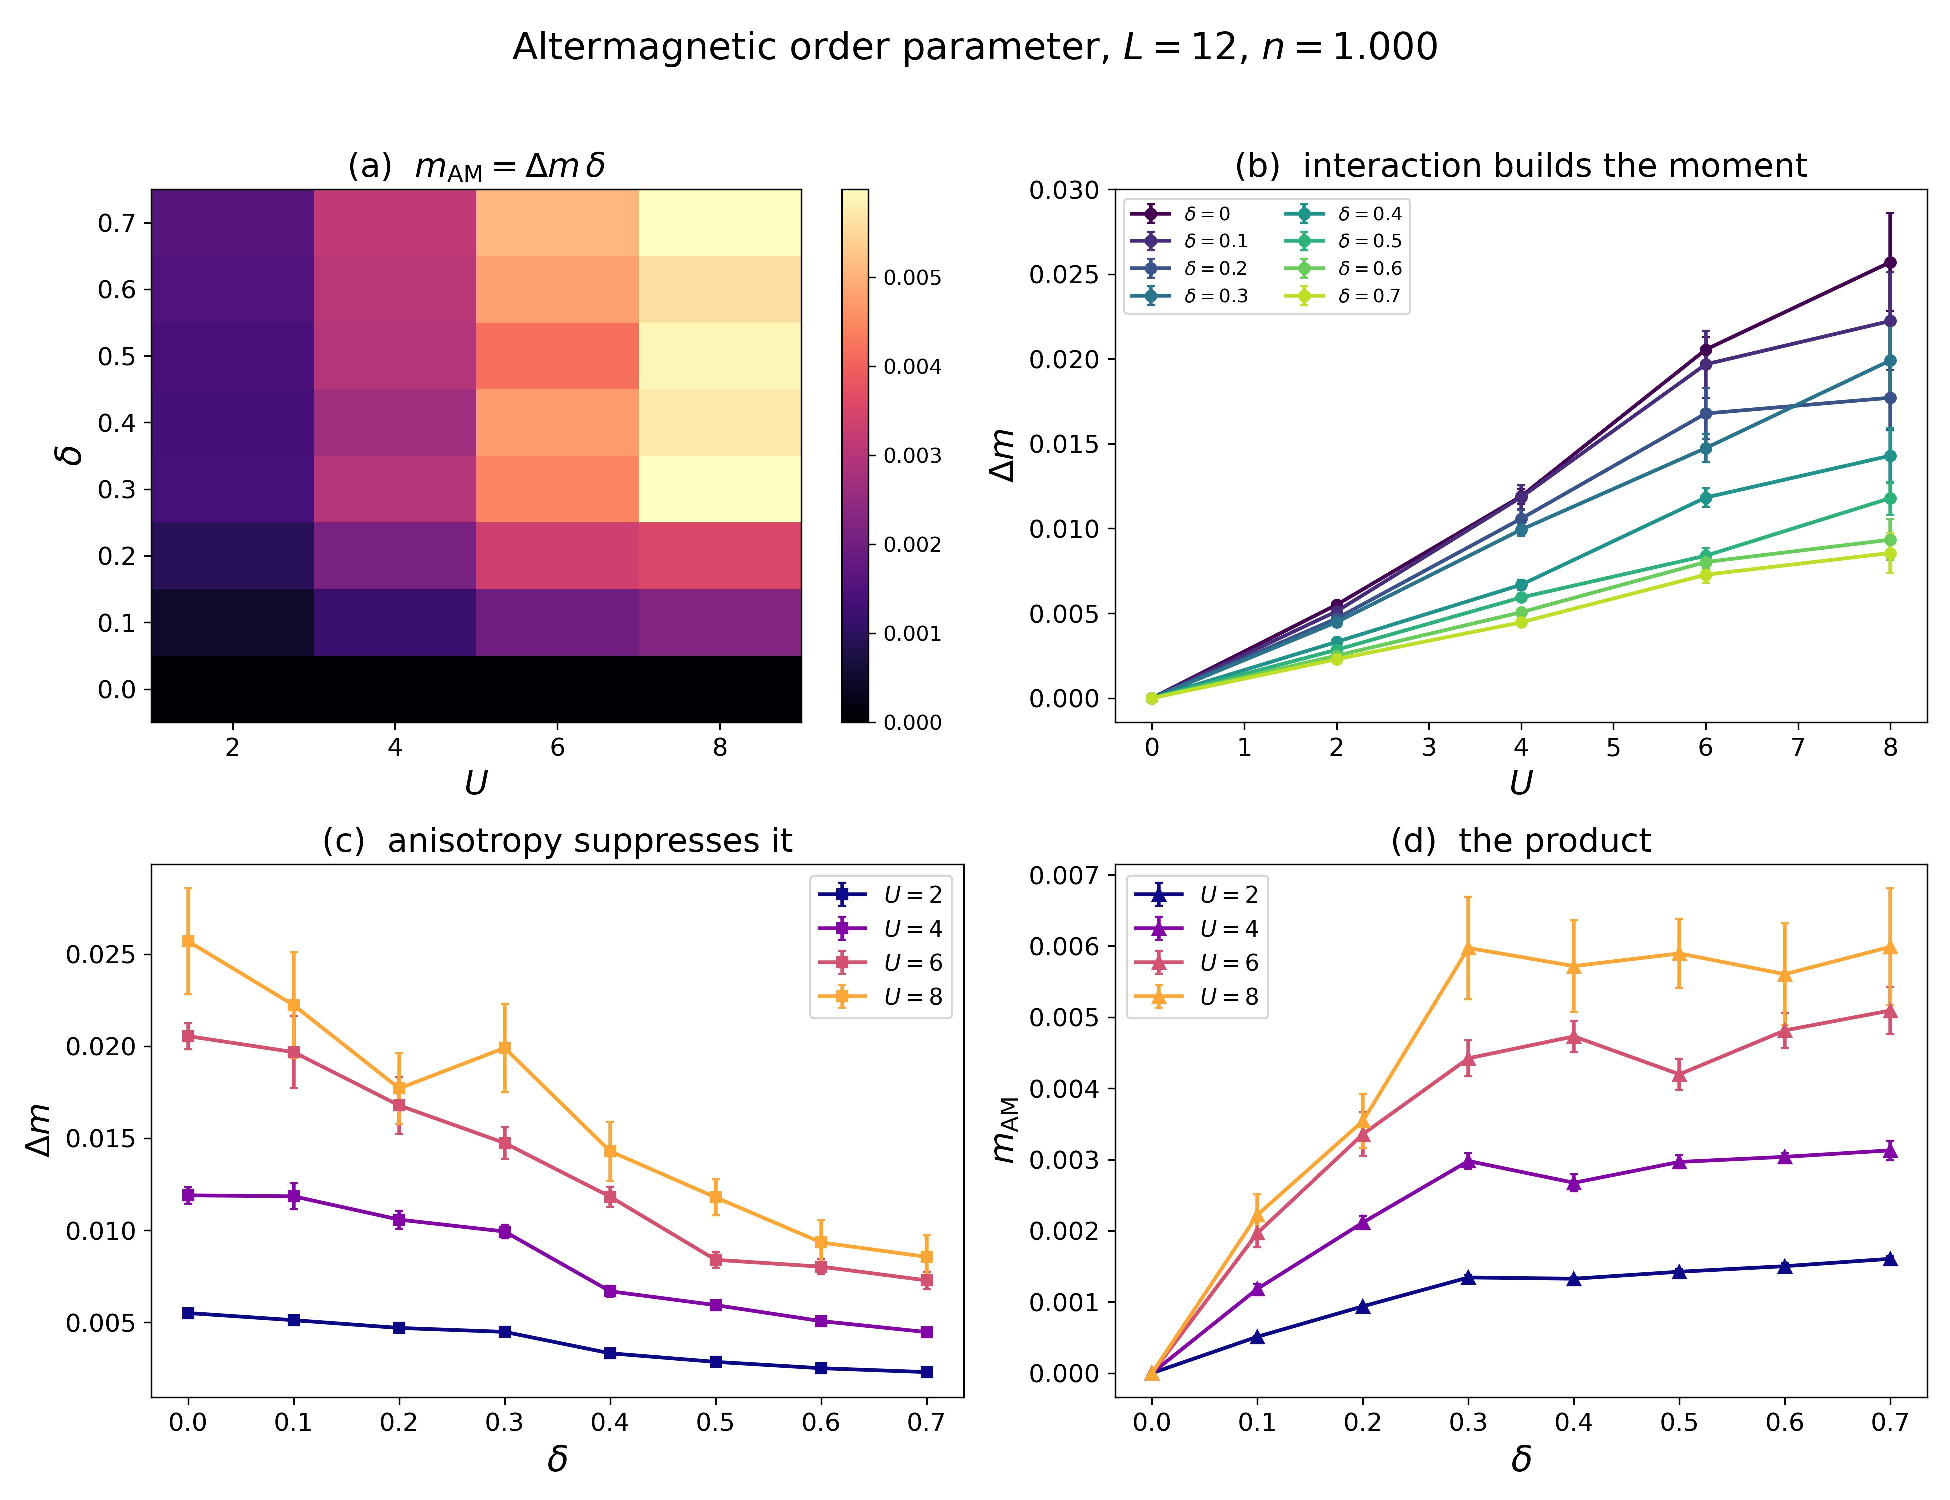
\includegraphics[width=\columnwidth]{fig_mAM_U_delta_L12.pdf}
\caption{Decomposition of the altermagnetic order parameter at $L = 12$ and half
filling. (a) $m_{\mathrm{AM}} = \Delta m\,\delta$ over the $(U,\delta)$ plane,
identically zero along $\delta = 0$. (b) The sublattice moment difference
$\Delta m$ against $U$ at fixed anisotropy, growing from zero in every case.
(c) $\Delta m$ against $\delta$ at fixed interaction, suppressed as the anisotropy
grows. (d) The product, which rises to $\delta \approx 0.3$ and is nearly flat
beyond it.}
\label{fig:mam}
\end{figure}

% ---------------------------------------------------------------------------
\section{Null control at vanishing anisotropy}
\label{sec:null}
% ---------------------------------------------------------------------------

Equation~(\ref{eq:dtot}) sums absolute values, so statistical noise contributes
with a definite sign and $\Delta_{\mathrm{tot}}$ has a positive floor that does
not vanish when the physics requires it to. Establishing the scale of that floor
requires a calculation in which the signal is forbidden but the sampling is
unchanged.

The $U = 0$ column does not serve this purpose. There the Green function is
obtained without auxiliary fields, so the zero is a matter of arithmetic rather
than of statistics and it tests nothing about the sampling.

At $\delta = 0$ both diagonal bonds are equal on every site, the two sublattices
become equivalent, and the model reduces to the square lattice with uniform
second-neighbor hopping. Its N\'eel sublattices are related by a translation, so
$n_{\uparrow}(\bm{k}) = n_{\downarrow}(\bm{k})$ identically and
$\Delta_{\mathrm{tot}}$ must vanish by symmetry at any $U$. Whatever is measured
there is the statistical floor at production settings.

We find $\Delta_{\mathrm{tot}}/N = 6.3(2)\times10^{-4}$, averaged over $U = 2$,
$3$, $3.5$, $4$, $4.5$, and $5$ at $L = 12$.
% data/delta0_control_L12.csv: 0.000626 +/- 0.000214
At $\delta = 0.3$ the measured signal ranges from $1.47\times10^{-2}$ at $U = 2$
to $7.13\times10^{-2}$ at $U = 4.5$, which is between $23$ and $114$ times this
floor.
% data/fortran_L12_all49.csv, delta=0.3

\begin{figure}[t]
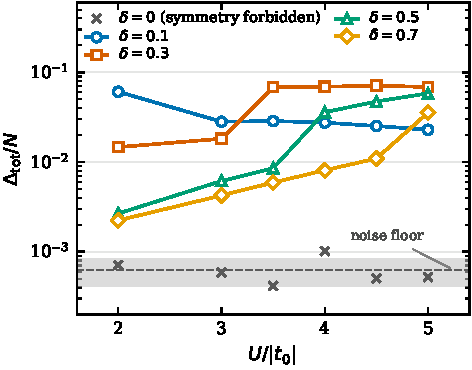
\includegraphics[width=\columnwidth]{fig05_null_control.pdf}
\caption{Null control. At $\delta = 0$ the splitting is forbidden by symmetry, so
the measured $\Delta_{\mathrm{tot}}/N$ there is the statistical floor at
production settings. The interacting signal at $\delta = 0.3$ sits between $23$
and $114$ times above it. The axis is logarithmic.}
\label{fig:null}
\end{figure}

% ---------------------------------------------------------------------------
\section{Finite-size behavior of the magnetic correlations}
\label{sec:fss}
% ---------------------------------------------------------------------------

The polarization of Sec.~\ref{sec:order} is measured on finite lattices, and a
nonzero value there does not by itself establish order in the thermodynamic
limit. We therefore examine two quantities that distinguish a genuine order
parameter from a finite-size remnant.

The first is the equal-time spin structure factor at the ordering wave vector,
$S(\pi,\pi)/N$. Across $L = 8$, $10$, and $12$ and for densities from $n = 0.5$
to $n = 1$ at $U$ up to $8$, the ratio between successive sizes falls between
$0.39$ and $0.54$, against $0.44$ for a pure $1/N$ decay. A structure factor that
scales as $1/N$ carries no long-range order, so this alone leaves the
correlations short ranged on the lattices reached here.

The second is the extrapolation of the staggered moment to vanishing field. The
$h \to 0$ intercept is nonzero at each individual size and decreases
monotonically with $L$, taking the values $0.03269$, $0.02363$, $0.01845$, and
$0.01714$ at $L = 8$, $10$, $12$, and $14$. On those four points alone the
extrapolation is ambiguous. A fit in $1/L^2$ gives $\chi^2/\mathrm{dof} = 2.1$
against $7.6$ for a fit in $1/L$, which favors a finite intercept and therefore
order.

The $L = 16$ calculation resolves the ambiguity. The two fits predict $0.01325$
in $1/L$ and $0.01457$ in $1/L^2$, and the measured value is
$0.00734 \pm 0.00109$. The drop from $L = 14$ is a factor of $0.43$ where a $1/L$
law predicts $0.88$, and including the point raises the $1/L^2$
$\chi^2/\mathrm{dof}$ from $2.1$ to $11.9$. Figure~\ref{fig:fss} shows both the
field scans and the extrapolation. The intercept is a finite-size effect and the
magnetic correlations remain short ranged.

\begin{figure}[t]
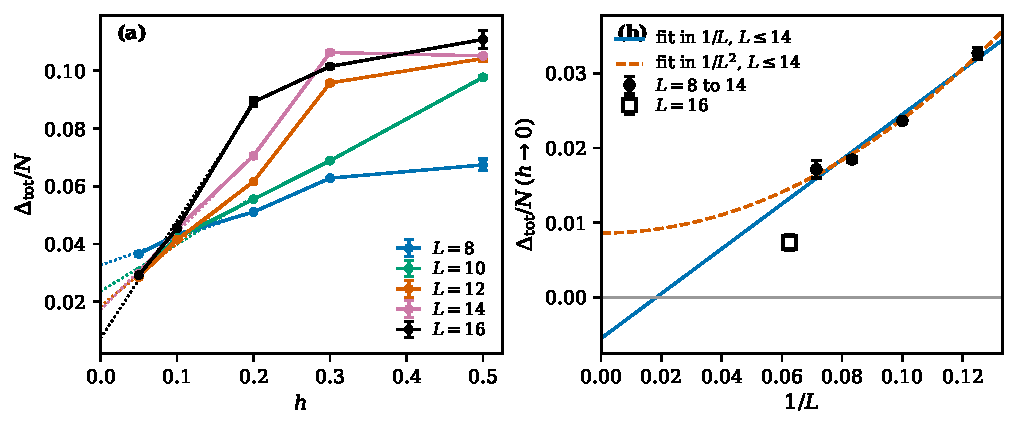
\includegraphics[width=\columnwidth]{fig06_fss_hscan.pdf}
\caption{(a) $\Delta_{\mathrm{tot}}/N$ against the staggered field $h$ for
$L = 8$ to $16$, with dotted lines giving the linear extrapolation to $h = 0$.
(b) The extrapolated intercept against $1/L$. Fits to $L \leq 14$ in $1/L$ and in
$1/L^2$ both overshoot the measured $L = 16$ point (open square), which falls
below either prediction.}
\label{fig:fss}
\end{figure}

This is a statement about the correlation length, not about the symmetry of the
polarization. The classification of Sec.~\ref{sec:order} rests on ratios of sums
over the Brillouin zone at a fixed lattice size, so it is unaffected by the
scaling of the correlation length.

% ---------------------------------------------------------------------------
\section{Pairing in the $d_{xy}$ channel}
\label{sec:pairing}
% ---------------------------------------------------------------------------

We compute the pair-field susceptibility in four channels, on-site $s$, extended
$s$, $d_{x^2-y^2}$, and $d_{xy}$, and separate the interaction-induced vertex
from the uncorrelated part. The vertex is the meaningful measure of whether the
interaction builds pairing, since the full correlator is large and positive
already for free electrons. The same separation underlies the long-running
question of whether the plain square-lattice Hubbard model superconducts at
all~\cite{Scalapino2012,Qin2020,Simkovic2024,Huang2019,Jiang2021}, and the study
of pairing driven by repulsion on other lattice
geometries~\cite{Nandkishore2012,Kiesel2012}. Figure~\ref{fig:eqvertex} contrasts
the two.

\begin{figure}[t]
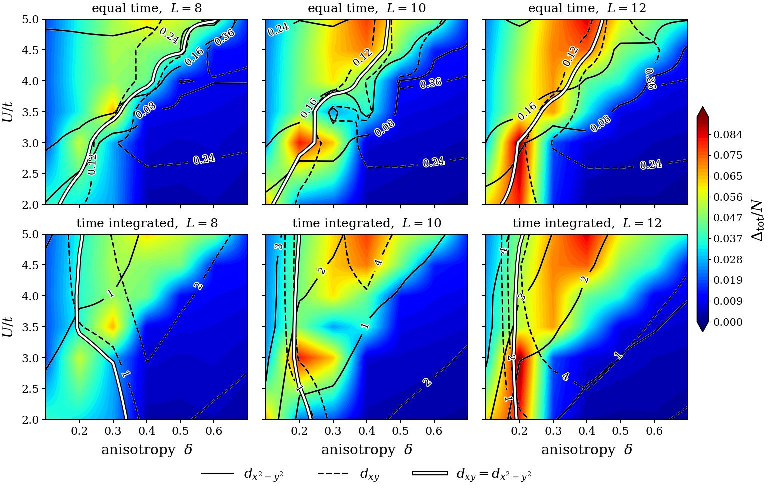
\includegraphics[width=\columnwidth]{fig_2row_eqtime_vertex_3L.pdf}
\caption{Equal-time correlator (top row) against the interaction-induced vertex
(bottom row) for $L = 8$, $10$, and $12$. The channel crossover straightens along
the vertex row, which is why the vertex rather than the full correlator is used
throughout.}
\label{fig:eqvertex}
\end{figure}

Three features stand out. The vertex is zero in all four channels at $U = 0$, so
everything that follows is interaction generated. The on-site $s$ vertex is
negative throughout, as a repulsive $U$ requires. The $d_{xy}$ vertex is the
largest of the four for $\delta \geq 0.3$ at every $U$ studied, and it grows
monotonically with $U$, from $3.347(8)$ at $U = 2$ to $5.952(22)$ at $U = 4.5$,
in both cases peaking at $\delta = 0.4$.
% data/chi_vertex_summary_3L.csv

The leading channel changes with anisotropy. For $\delta \leq 0.2$ the extended
$s$ channel is largest and for $\delta \geq 0.3$ the $d_{xy}$ channel is.
Figure~\ref{fig:ddiff} shows the difference between the two $d$ channels directly
across three sizes.

\begin{figure}[t]
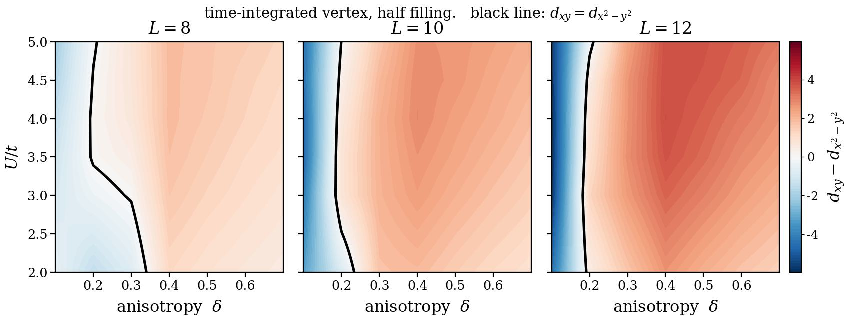
\includegraphics[width=\columnwidth]{fig_ddiff_vertex_3L.pdf}
\caption{Difference between the $d_{xy}$ and $d_{x^2-y^2}$ vertices over the
$(U,\delta)$ plane at $L = 8$, $10$, and $12$. The white contour marks where the
two are equal. $d_{xy}$ leads everywhere to its right, and the boundary moves
very little with size.}
\label{fig:ddiff}
\end{figure}

% ---------------------------------------------------------------------------
\section{Size dependence of the pairing vertex}
\label{sec:vertexfss}
% ---------------------------------------------------------------------------

The vertex was computed at $L = 8$, $10$, and $12$ under identical settings,
which allows the anisotropy of the channel crossover to be followed with size.

The crossover anisotropy $\delta_c$, defined as the value at which the $d_{xy}$
vertex overtakes the extended $s$ vertex, is nearly independent of $U$ and
becomes more so as the lattice grows. Its spread across the six interaction
strengths studied is $0.148$ at $L = 8$, $0.049$ at $L = 10$, and $0.028$ at
$L = 12$, and the mean value moves from $0.235$ to $0.197$ to $0.192$. A
crossover set by the interaction strength would not converge in this way, so we
read $\delta_c \approx 0.19$ as a property of the lattice geometry.
% code/check_vertex_fss.py

The $d_{xy}$ vertex grows with system size at every interaction strength, by a
factor between $2.18$ and $2.38$ from $L = 8$ to $L = 12$. The $d_{x^2-y^2}$
vertex is positive in all $126$ cells at all three sizes, so that channel is
never repulsive even where it is subdominant. The optimal anisotropy for $d_{xy}$
is $\delta = 0.4$ at essentially every size and interaction strength.
Figure~\ref{fig:pairfss} collects these three statements.

\begin{figure}[t]
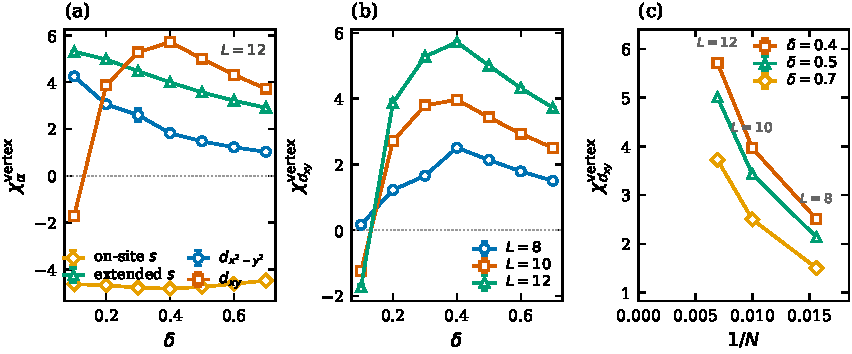
\includegraphics[width=\columnwidth]{fig09_pairing_fss.pdf}
\caption{Interaction-induced pairing vertex at half filling, $U = 4$. (a) The
four channels against $\delta$ at $L = 12$. (b) The $d_{xy}$ vertex against
$\delta$ for three sizes. (c) The $d_{xy}$ vertex against $1/N$ at three
anisotropies, growing with system size in every case.}
\label{fig:pairfss}
\end{figure}

Magnetism and pairing move together rather than merely coexisting. With $\delta$
and $U$ both partialled out, the correlation between the pairing vertex and
$\Delta_{\mathrm{tot}}$ is $+0.57$ in the $d_{xy}$ channel and $-0.51$ in the
$d_{x^2-y^2}$ channel.
% code/check_pairing_vs_dtot.py
The two channels respond to the magnetic signal with opposite sign at fixed
anisotropy and fixed interaction. Figure~\ref{fig:overlay} places the pairing
contours directly on the magnetic map.

\begin{figure}[t]
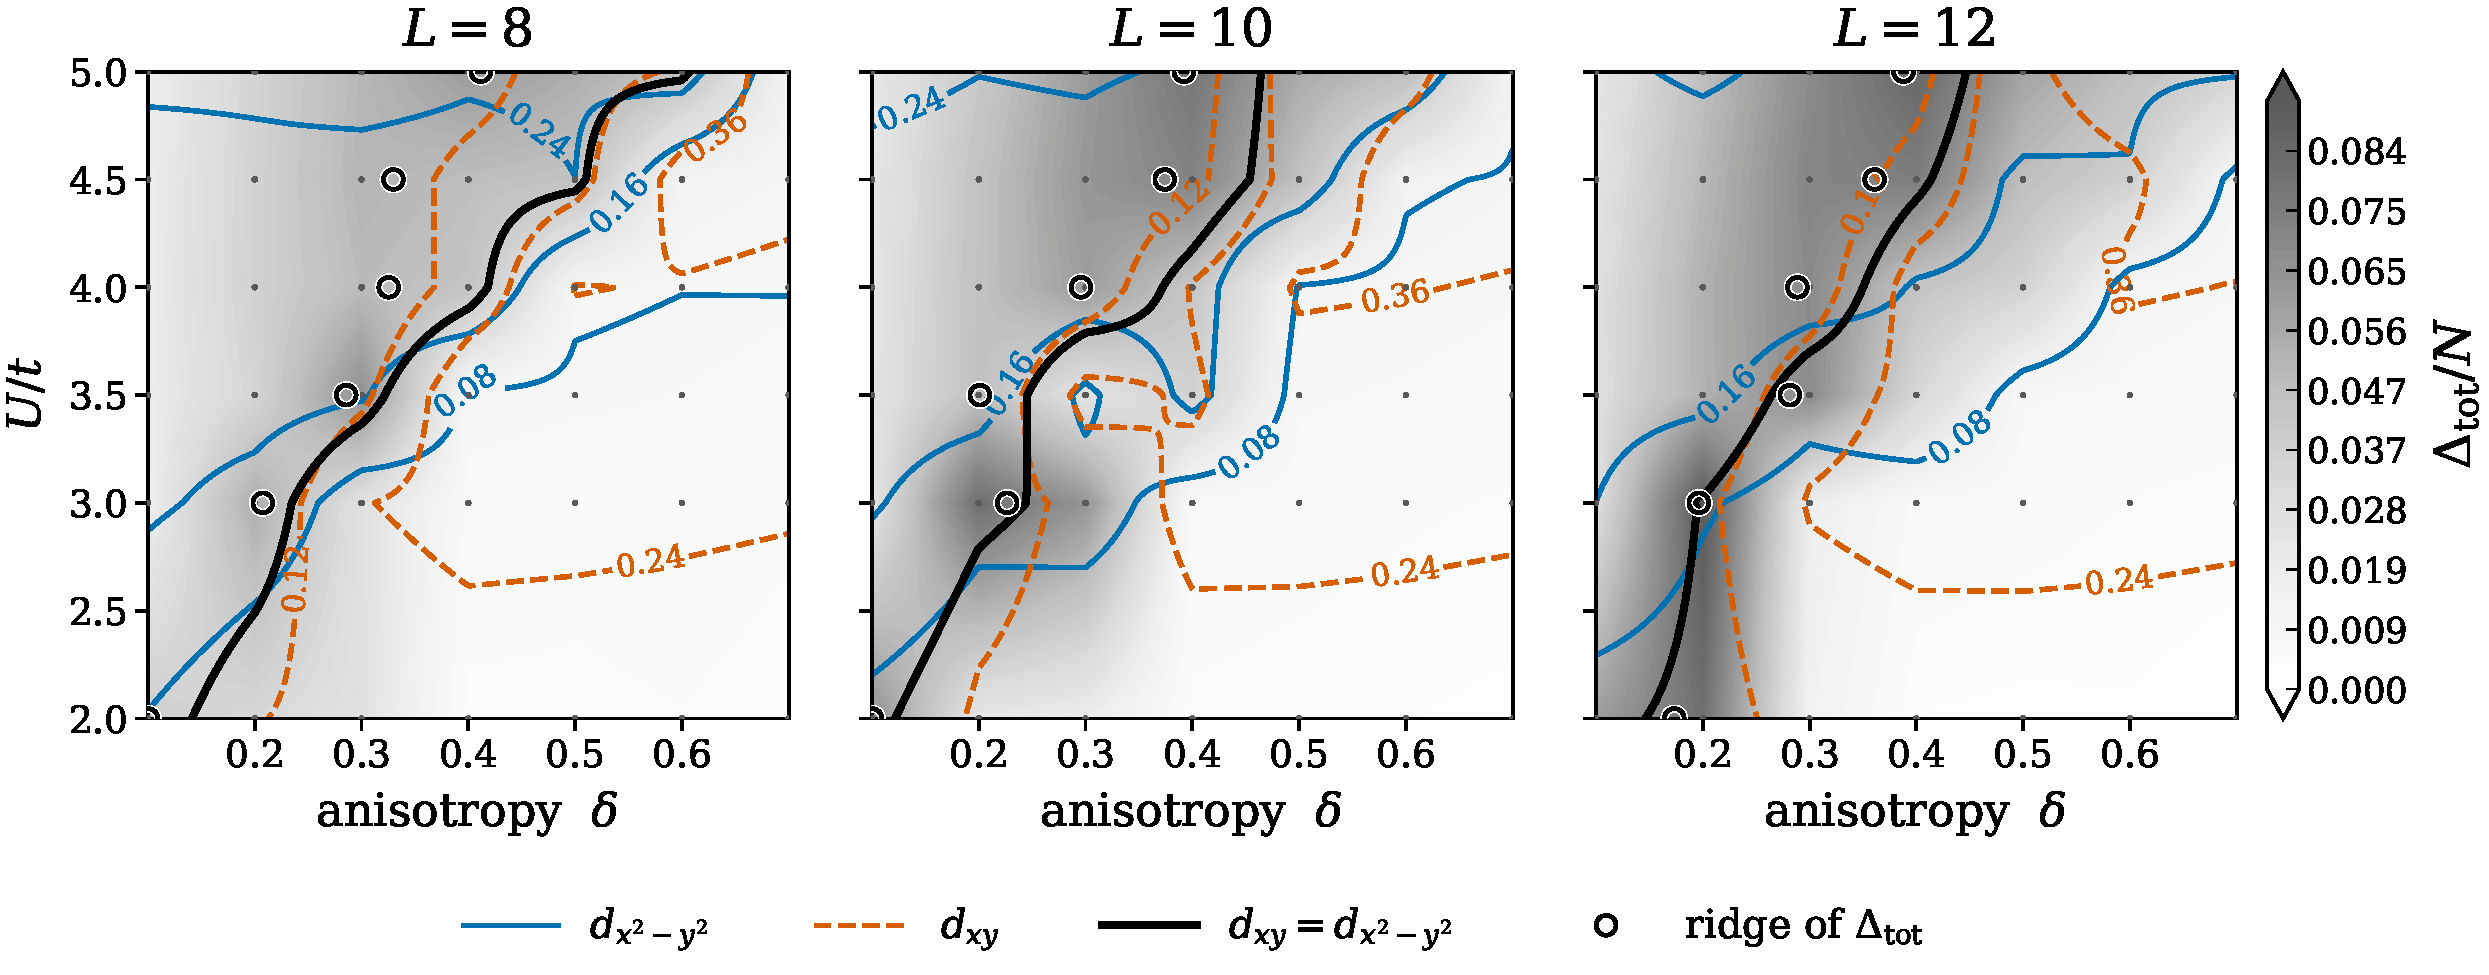
\includegraphics[width=\columnwidth]{fig_dchannels_over_dtot.pdf}
\caption{Pairing channel contours over the magnetic polarization. The background
is $\Delta_{\mathrm{tot}}/N$ and the contours are the two $d$ vertices, with the
white line marking where they cross. The crossover tracks the ridge of the
magnetic signal rather than cutting across it.}
\label{fig:overlay}
\end{figure}

The magnetic and pairing instabilities therefore select the same representation.
The polarization is $d_{xy}$ at all 126 parameter sets, and the pairing vertex is
largest in $d_{xy}$ over the anisotropy range where that classification holds
most strongly.

% ---------------------------------------------------------------------------
\section{Robustness and comparison}
\label{sec:robust}
% ---------------------------------------------------------------------------

At half filling with periodic boundaries the noninteracting spectrum of
Eq.~(\ref{eq:H}) is gapless at every $L$ and $\delta$ we examined, so the
occupied set is fixed by the trial state rather than by the spectrum.
Appendix~\ref{app:bc} reports a repeat with antiperiodic boundaries, which shift
the momentum mesh off the high-symmetry points and open a gap. The two agree on
the sign of $\partial \Delta_{\mathrm{tot}} / \partial U$ at $\delta = 0.1$ and
$\delta = 0.5$ and disagree at $\delta = 0.3$, which we read as the anisotropy
where the slope passes through zero. We therefore do not quote a slope there.

The closest published work is a determinant quantum Monte Carlo study of the
checkerboard Hubbard model that reports $d$-wave and $d + is$ pairing as the
dominant channels~\cite{Pan2024}. The two Hamiltonians are not the same. That
model keeps one diagonal per sublattice and omits the other, whereas
Eq.~(\ref{eq:H}) keeps both, and the two coincide only where our second diagonal
vanishes, at $\delta = t_1 = 0.3$. We verified that the single-particle spectra
agree there to within $4\times10^{-15}$.

At that point, and at half filling, we evaluated the vertex in the basis of
Ref.~\cite{Pan2024} alongside our own. Within their basis the $s$-wave channel is
the larger of the two at $U = 3$, $4$, and $4.5$. Including $d_{xy}$, which their
basis does not contain, gives a $d_{xy}$ vertex larger than either.
% data/pan, analyze_pan.py
The comparison is restricted, since Ref.~\cite{Pan2024} works at density
$n = 0.9$ and temperature $T/t = 1/6$ while our calculations are at half filling
in the ground state, and under the particle-hole transformation that relates the
two signs of the second-neighbor hopping their density maps to $n = 1.1$. The
statement is that the dominant channel we find lies outside the basis used there,
not that the two calculations disagree.

% ---------------------------------------------------------------------------
\section{Conclusion}
% ---------------------------------------------------------------------------

The half-filled checkerboard Hubbard model supports compensated spin-split
correlations that are absent at $U = 0$ and are $d_{xy}$ in symmetry at every
parameter set examined. A control at vanishing anisotropy, where the splitting is
forbidden, places the statistical floor two orders of magnitude below the signal.
The interaction-induced pairing vertex is largest in the same $d_{xy}$ channel,
and the anisotropy at which the pairing channel changes coincides with the
anisotropy at which the magnetic response changes sign.

The mechanism uses no spin-dependent hopping and no spin-orbit coupling. It
requires only a lattice whose magnetic sublattices are related by a rotation and a
uniform Hubbard repulsion, which suggests that the same construction should apply
to other lattices with the same sublattice relation. Whether the state survives to
the thermodynamic limit is not settled by the sizes reached here, and the
constrained-path bias remains.

\appendix

% ---------------------------------------------------------------------------
\section{Trial wave function and the selection of the constrained path}
\label{app:trial}
% ---------------------------------------------------------------------------

The constrained-path approximation replaces the sign problem with a bias fixed by
the trial wave function, so the trial is part of the method rather than an
implementation detail. We take the trial from an unrestricted Hartree-Fock
solution of Eq.~(\ref{eq:H}) at the same $U$, $\delta$, and filling, and we select
among the solutions reached from different starting densities by the variational
energy
\begin{equation}
E_{\mathrm{HF}} = \mathrm{Tr}\,(K \rho_{\uparrow}) + \mathrm{Tr}\,(K \rho_{\downarrow})
                + U \sum_i \langle n_{i\uparrow}\rangle \langle n_{i\downarrow}\rangle ,
\label{eq:ehf}
\end{equation}
with $\rho_{\sigma} = V_{\sigma} V_{\sigma}^{\dagger}$ built from the occupied
columns of the mean-field eigenvectors and $K$ the one-body matrix of
Eq.~(\ref{eq:H}).

Equation~(\ref{eq:ehf}) is not interchangeable with the sum of mean-field
eigenvalues. Each eigenvalue already contains the mean field of the opposite
spin, so that sum counts the interaction twice and orders competing solutions
differently from the energy. The two criteria can select different states, and
because the constrained path is fixed by whichever state is chosen, the selection
propagates into every measured quantity. At half filling the state chosen by the
eigenvalue sum carries the larger staggered moment in every case where the two
differ, so the criterion matters for exactly the quantity under study. We report
results obtained with Eq.~(\ref{eq:ehf}) throughout.

The identity
$E_{\mathrm{HF}} = \sum_p \varepsilon_p - U \sum_i \langle n_{i\uparrow}\rangle
\langle n_{i\downarrow}\rangle$
holds only at exact self consistency and should not be substituted for
Eq.~(\ref{eq:ehf}). A mean-field iteration that mixes densities between steps does
not reach that condition for loosely converged solutions, which are precisely the
ones whose ranking is at issue.

% ---------------------------------------------------------------------------
\section{Convergence in projection length}
\label{app:beta}
% ---------------------------------------------------------------------------

All results use a projection length $\beta = 32$ in units of $1/|t_0|$. Doubling
it to $\beta = 48$ at otherwise identical settings changes the order parameter by
between $0.1\%$ and $4.1\%$ with no systematic drift in either direction, which we
take as convergence.

% ---------------------------------------------------------------------------
\section{Boundary conditions}
\label{app:bc}
% ---------------------------------------------------------------------------

Antiperiodic boundaries shift the momentum mesh off the high-symmetry points and
open a gap in the noninteracting spectrum. The sign of
$\partial \Delta_{\mathrm{tot}} / \partial U$ agrees between the two choices at
$\delta = 0.1$, where both are negative, and at $\delta = 0.5$, where both are
positive, with magnitudes matching to within a few percent. At $\delta = 0.3$ the
two disagree and the antiperiodic value is consistent with zero. We read
$\delta \approx 0.3$ as the anisotropy at which the slope passes through zero,
where its sign is most sensitive to the mesh, and we do not quote a slope there.
% data/bc_test, analyze_bc_test.py

\begin{acknowledgments}
% TODO: funding and computing acknowledgments.
\end{acknowledgments}

\begin{thebibliography}{99}

% Bibliography generated by code/make_bibliography.py from Crossref records.
% Every entry below carries a registered DOI. The two hand entries are the
% group's own PRB and a preprint, neither of which had a usable record.

\bibitem{Hubbard1963}
J.~Hubbard,
Proc. R. Soc. London Ser. A \textbf{276}, 238 (1963).

\bibitem{BSS1981}
D.~Scalapino, and R.~Sugar,
Phys. Rev. B \textbf{24}, 4295 (1981).

\bibitem{Hirsch1983}
J.~Hirsch,
Phys. Rev. B \textbf{28}, 4059 (1983).

\bibitem{Hirsch1985}
J.~Hirsch,
Phys. Rev. B \textbf{31}, 4403 (1985).

\bibitem{Lieb1989}
E.~Lieb,
Phys. Rev. Lett. \textbf{62}, 1201 (1989).

\bibitem{Sorella1989}
S.~Sorella, S.~Baroni, R.~Car, and M.~Parrinello,
Europhys. Lett. \textbf{8}, 663 (1989).

\bibitem{Loh1990}
E.~Loh \textit{et al.},
Phys. Rev. B \textbf{41}, 9301 (1990).

\bibitem{Mielke1991}
A.~Mielke,
J. Phys. A \textbf{24}, 3311 (1991).

\bibitem{Tasaki1992}
H.~Tasaki,
Phys. Rev. Lett. \textbf{69}, 1608 (1992).

\bibitem{Zhang1997}
S.~Zhang, J.~Carlson, and J.~Gubernatis,
Phys. Rev. B \textbf{55}, 7464 (1997).

\bibitem{ZhangKrakauer2003}
S.~Zhang, and H.~Krakauer,
Phys. Rev. Lett. \textbf{90}, 136401 (2003).

\bibitem{Troyer2005}
M.~Troyer, and U.~Wiese,
Phys. Rev. Lett. \textbf{94}, 170201 (2005).

\bibitem{Varney2009}
C.~Varney \textit{et al.},
Phys. Rev. B \textbf{80}, 075116 (2009).

\bibitem{Scalapino2012}
D.~Scalapino,
Rev. Mod. Phys. \textbf{84}, 1383 (2012).

\bibitem{Nandkishore2012}
R.~Nandkishore, L.~Levitov, and A.~Chubukov,
Nat. Phys. \textbf{8}, 158 (2012).

\bibitem{Kiesel2012}
M.~Kiesel \textit{et al.},
Phys. Rev. B \textbf{86}, 020507 (2012).

\bibitem{LeBlanc2015}
J.~LeBlanc \textit{et al.},
Phys. Rev. X \textbf{5}, 041041 (2015).

\bibitem{Qin2016}
M.~Qin, H.~Shi, and S.~Zhang,
Phys. Rev. B \textbf{94}, 085103 (2016).

\bibitem{Huang2019}
E.~Huang, R.~Sheppard, B.~Moritz, and T.~Devereaux,
Science \textbf{366}, 987 (2019).

\bibitem{Qin2020}
M.~Qin \textit{et al.},
Phys. Rev. X \textbf{10}, 031016 (2020).

\bibitem{SmejkalCrystal}
L.~Šmejkal, R.~González-Hernández, T.~Jungwirth, and J.~Sinova,
Sci. Adv. \textbf{6}, eaaz8809 (2020).

\bibitem{Jiang2021}
Y.~Jiang, J.~Zaanen, T.~Devereaux, and H.~Jiang,
Phys. Rev. Research \textbf{2}, 033073 (2020).

\bibitem{Mazin2021}
I.~Mazin \textit{et al.},
Proc. Natl. Acad. Sci. U.S.A. \textbf{118}, e2108924118 (2021).

\bibitem{Smejkal2022a}
L.~Šmejkal, J.~Sinova, and T.~Jungwirth,
Phys. Rev. X \textbf{12}, 031042 (2022).

\bibitem{Smejkal2022b}
L.~Šmejkal, J.~Sinova, and T.~Jungwirth,
Phys. Rev. X \textbf{12}, 040501 (2022).

\bibitem{Feng2022}
Z.~Feng \textit{et al.},
Nat. Electron. \textbf{5}, 735 (2022).

\bibitem{Arovas2022}
D.~Arovas, E.~Berg, S.~Kivelson, and S.~Raghu,
Annu. Rev. Condens. Matter Phys. \textbf{13}, 239 (2022).

\bibitem{Brekke2023}
B.~Brekke, A.~Brataas, and A.~Sudbø,
Phys. Rev. B \textbf{108}, 224421 (2023).

\bibitem{Ouassou2023}
J.~Ouassou, A.~Brataas, and J.~Linder,
Phys. Rev. Lett. \textbf{131}, 076003 (2023).

\bibitem{Zhu2023}
D.~Zhu, Z.~Zhuang, Z.~Wu, and Z.~Yan,
Phys. Rev. B \textbf{108}, 184505 (2023).

\bibitem{Simkovic2024}
R.~Ma, and T.~Ma,
Phys. Rev. B \textbf{107}, 214509 (2023).

\bibitem{Bai2024}
L.~Bai \textit{et al.},
Adv. Funct. Mater. \textbf{34}, 2409327 (2024).

\bibitem{Krempasky2024}
J.~Krempaský \textit{et al.},
Nature \textbf{626}, 517 (2024).

\bibitem{Lee2024}
S.~Lee \textit{et al.},
Phys. Rev. Lett. \textbf{132}, 036702 (2024).

\bibitem{Reimers2024}
S.~Reimers \textit{et al.},
Nat. Commun. \textbf{15}, 2116 (2024).

\bibitem{Fedchenko2024}
O.~Fedchenko \textit{et al.},
Sci. Adv. \textbf{10}, eadj4883 (2024).

\bibitem{Leeb2024}
V.~Leeb, A.~Mook, L.~Šmejkal, and J.~Knolle,
Phys. Rev. Lett. \textbf{132}, 236701 (2024).

\bibitem{Roig2024}
M.~Roig \textit{et al.},
Phys. Rev. B \textbf{110}, 144412 (2024).

\bibitem{Chakraborty2024}
Q.~Cheng, Y.~Mao, and Q.~Sun,
Phys. Rev. B \textbf{110}, 014518 (2024).

\bibitem{Bhowal2024}
S.~Bhowal, and N.~Spaldin,
Phys. Rev. X \textbf{14}, 011019 (2024).

\bibitem{McClarty2024}
P.~McClarty, and J.~Rau,
Phys. Rev. Lett. \textbf{132}, 176702 (2024).

\bibitem{Duerrnagel2025}
M.~Dürrnagel \textit{et al.},
Phys. Rev. Lett. \textbf{135}, 036502 (2025).

\bibitem{Kaushal2025}
N.~Kaushal, and M.~Franz,
Phys. Rev. Lett. \textbf{135}, 156502 (2025).

\bibitem{Hariki2025}
D.~Takegami \textit{et al.},
Phys. Rev. Lett. \textbf{135}, 196502 (2025).

\bibitem{OurPRB}
Y.~Li \textit{et al.},
Phys. Rev. B \textbf{113}, 134443 (2026).

\bibitem{Pan2024}
Y.~Pan, R.~Ma, C.~Chen, Z.~Jia, and T.~Ma,
arXiv:2409.16523.

\end{thebibliography}

\end{document}
